\begin{frame}[t]{Key Concepts}

    \vskip .5cm
    
    % \begin{enumerate}[<+->]
    \begin{enumerate}
        \item \textbf{Communication Protocols:} Mappings from concepts to symbols
        \item \textbf{Intra-episodic Protocol Establishment}: agents enter into an environment without a shared protocol, but develop a protocol together within an episode
        \item \textbf{Zero-shot Communication:} Two strangers that have never met are able to communicate on their first interaction (within their first episode together)
    \end{enumerate}

\end{frame}

\begin{frame}[t]{Key Idea}

    \vskip 0.8cm
    
    \begin{center}
    \emph{
        Randomly exposing agents to different protocols during \\
        training should encourage the development of skills related \\
        to communicating with strangers
    }
    \vskip 0.2cm
    
    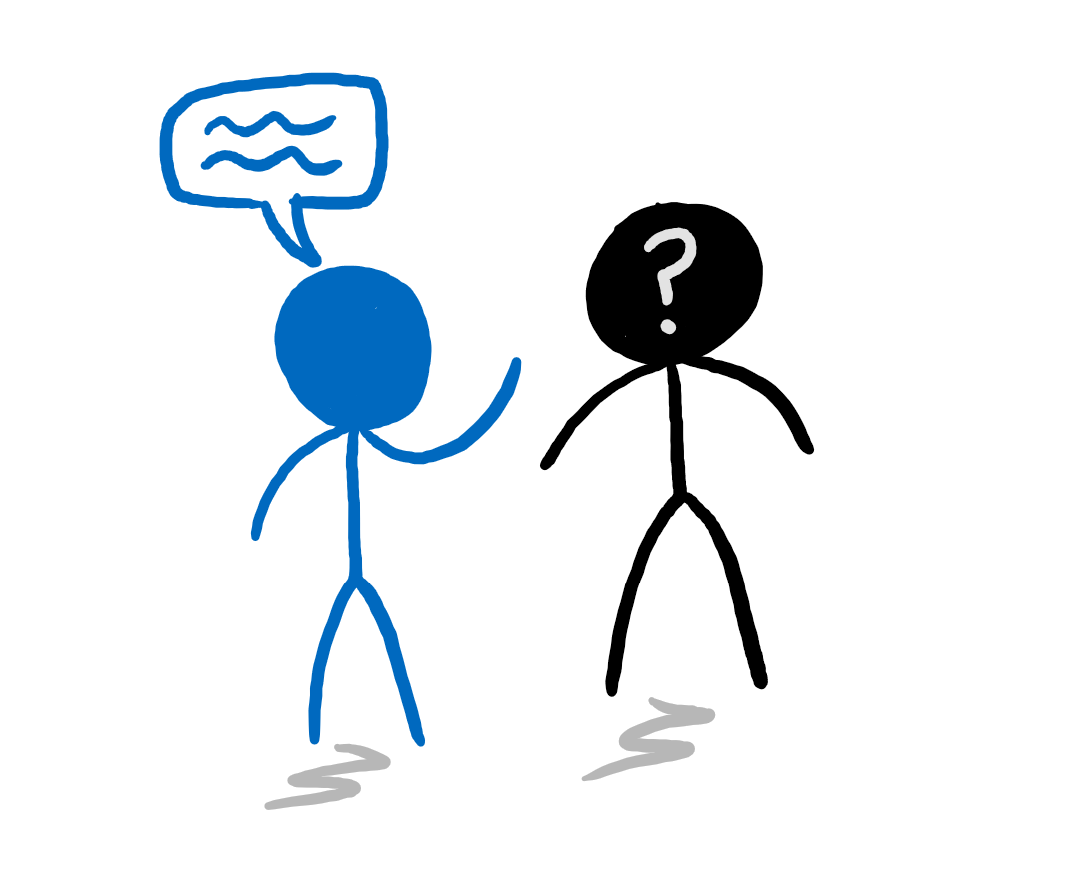
\includegraphics[width=0.5\linewidth]{figures/taking_to_stranger.png}
    
    \end{center}

\end{frame}

\begin{frame}{Our Environment}
    
    \centering
    % \vspace{-0.3cm}
    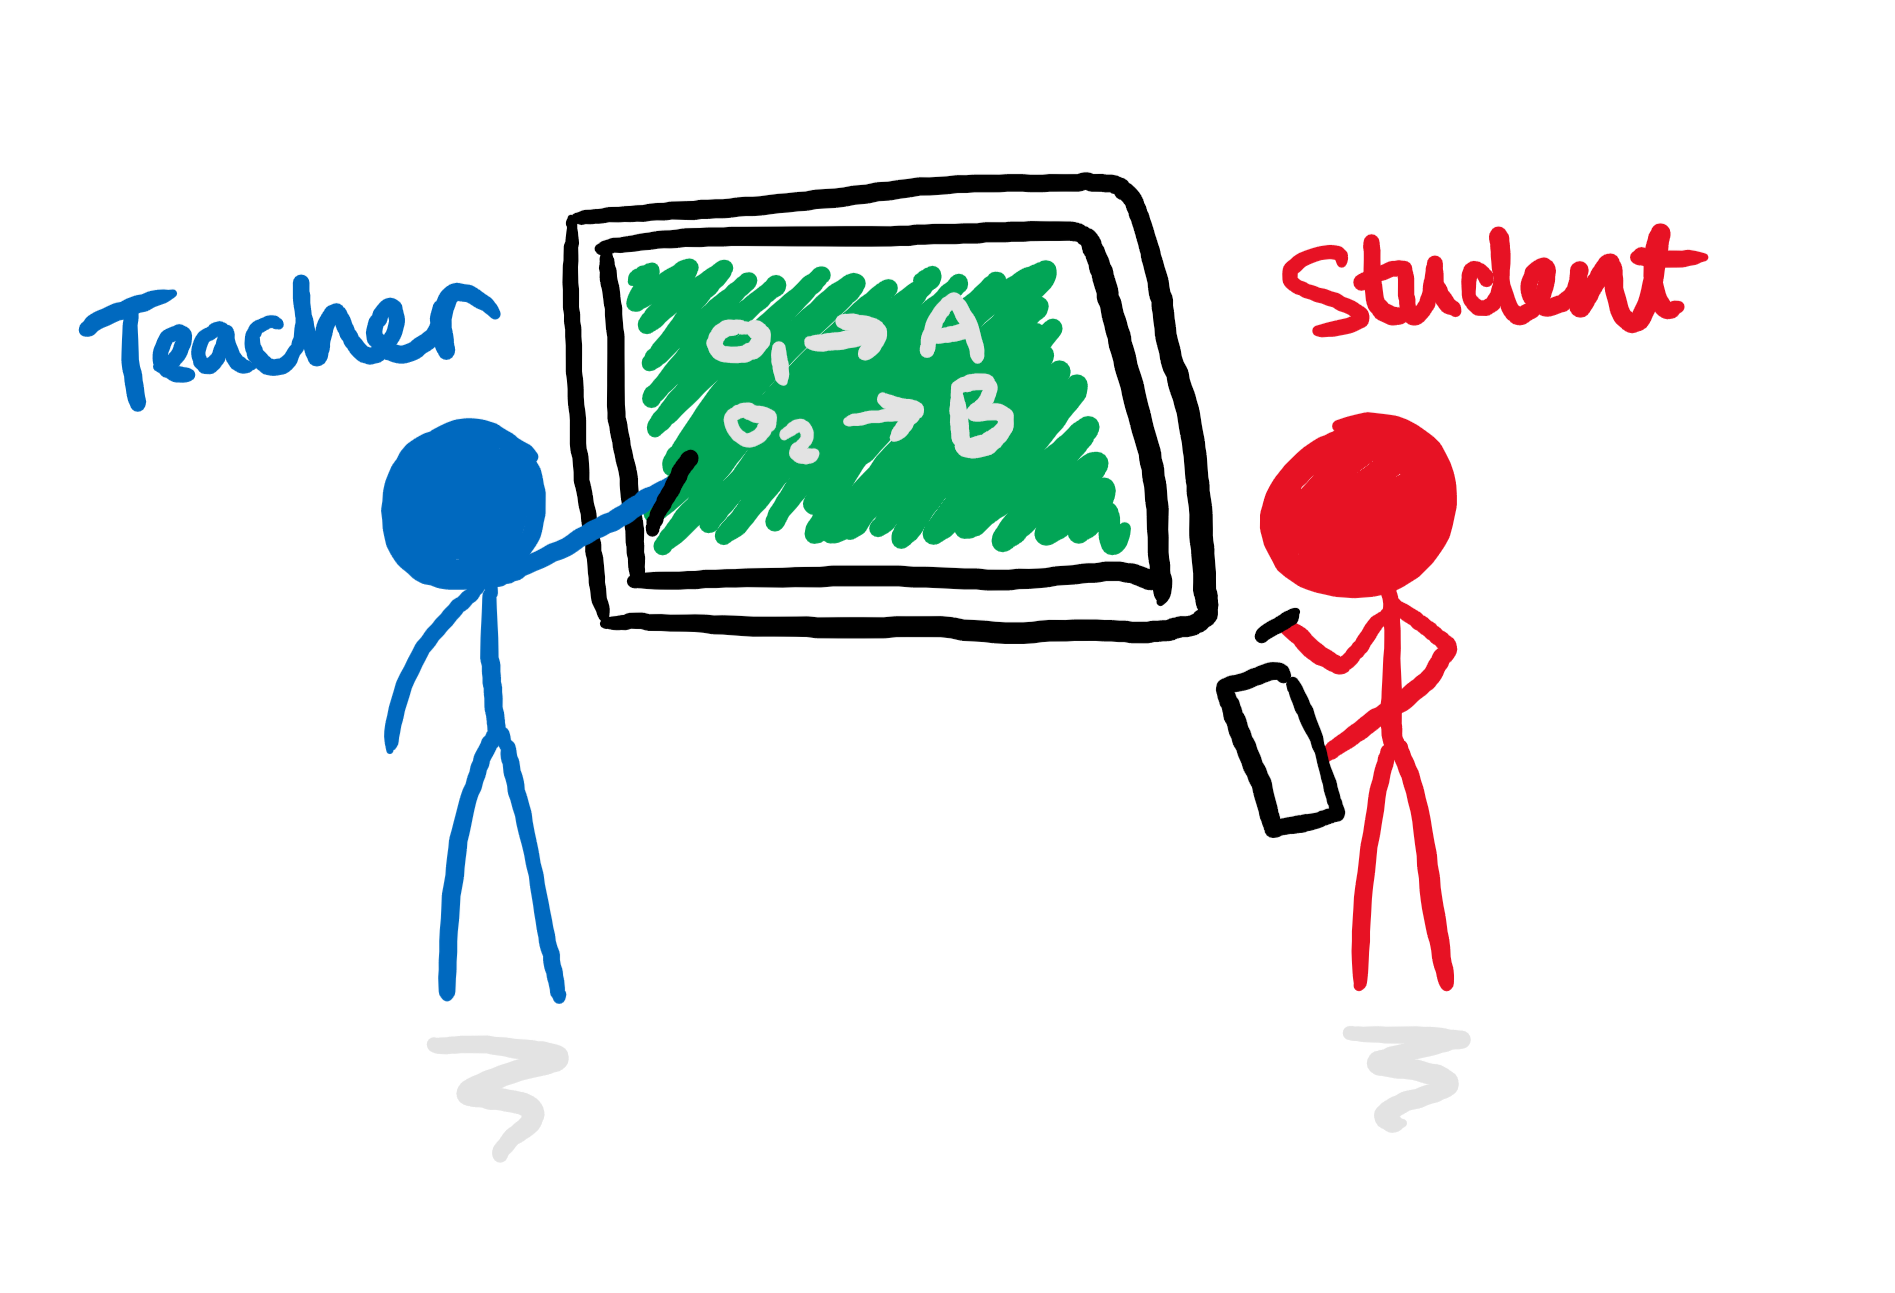
\includegraphics[width=0.6\linewidth]{figures/teacher_student_cartoon.png}
    \vspace{-0.3cm}
    
    \begin{enumerate}
        \item Teacher and student are both shown a series of inputs
        \item The teacher makes utterances
        \item The teacher is shown an input that is hidden from the student
        \item The agents are jointly rewarded based on the accuracy of student's prediction of the hidden input
    \end{enumerate}
    
\end{frame}

\begin{frame}{Our Environment}
    
    \begin{figure}
        \centering
        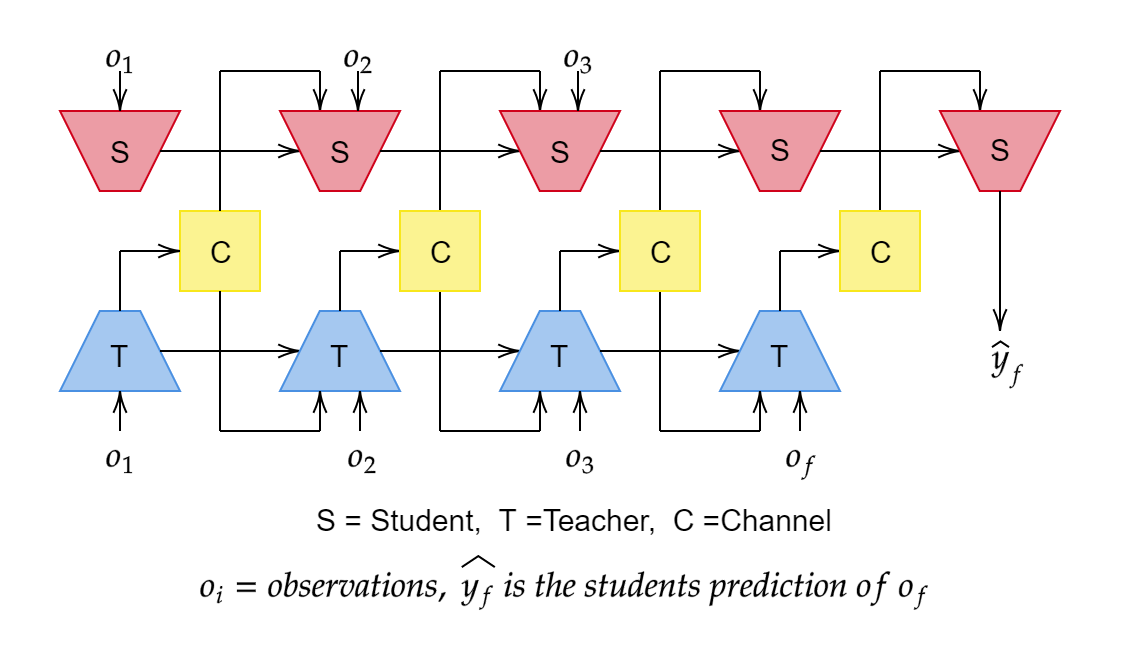
\includegraphics[width=1\linewidth]{figures/arch_diagram_red_blue.png}
        \caption{A diagram showing information flow through an episode}
        \label{fig:arch_diagram}
    \end{figure}
    
\end{frame}

\begin{frame}{Message Mutation}

    % TODO: Replace this slide with graphical representation

    The first of our proposals for improving zero-shot communication is \emph{message mutation}. This is a function $f_m : \Sigma \rightarrow \Sigma$ defined as follows: 
    \begin{equation}
    \begin{gathered}
    f_m(s) = \begin{cases}
        s' & \text{if}~x < p_m \\
        s & \text{otherwise}
    \end{cases} \\
    \text{where}~x\sim \text{Uniform}([0, 1]) ~\text{and}~ s' \sim \text{Uniform}(S).
    \end{gathered}
    \end{equation}
    
    \begin{center}
        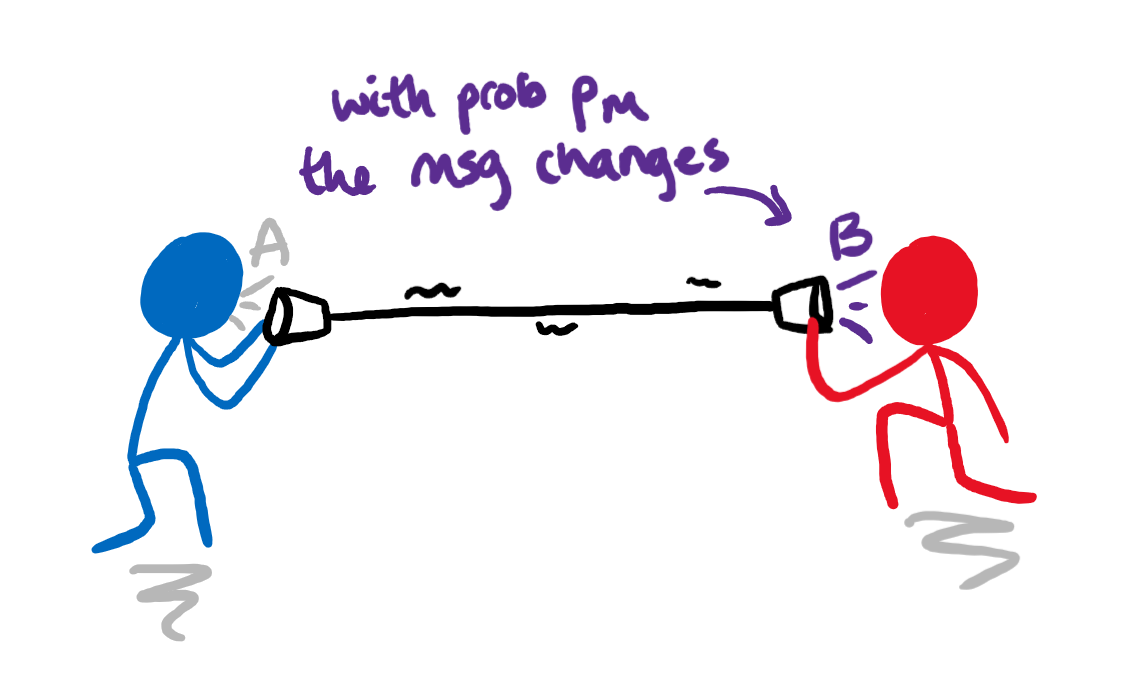
\includegraphics[width=0.6\linewidth]{figures/msg_mutation_cartoon.png}
    \end{center}
    
    
\end{frame}

\begin{frame}{Message Mutation}
    
    \begin{figure}
        \centering
        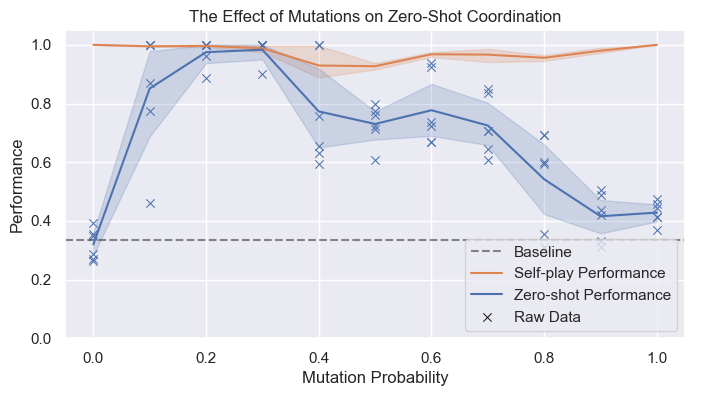
\includegraphics[width=1\linewidth]{figures/p_mutate_and_zs_coordination.png}
        \caption{Results with varying mutation probability}
        \label{fig:arch_diagram}
    \end{figure}
    
\end{frame}

\begin{frame}{Channel Permutation}

    % TODO: Replace this slide with graphical representation
    
    The second of our proposals is \textit{channel permutation}.
    
    For each episode an arbitrary bijective total function $f_{ij}: \Sigma \rightarrow \Sigma$, is created for every possible ordered pair of agents $i$ and $j$. Given the symmetric group $S_{|\Sigma|}$:
    \begin{align}
        f_{ij} \sim \text{Uniform}(S_{|\Sigma|}).   
    \end{align}
    Consequently, whenever agent $i$ sends a symbol $s \in \Sigma$ to agent $j$, agent $j$ receives $f_{ij}(s)$.
    
    \begin{center}
        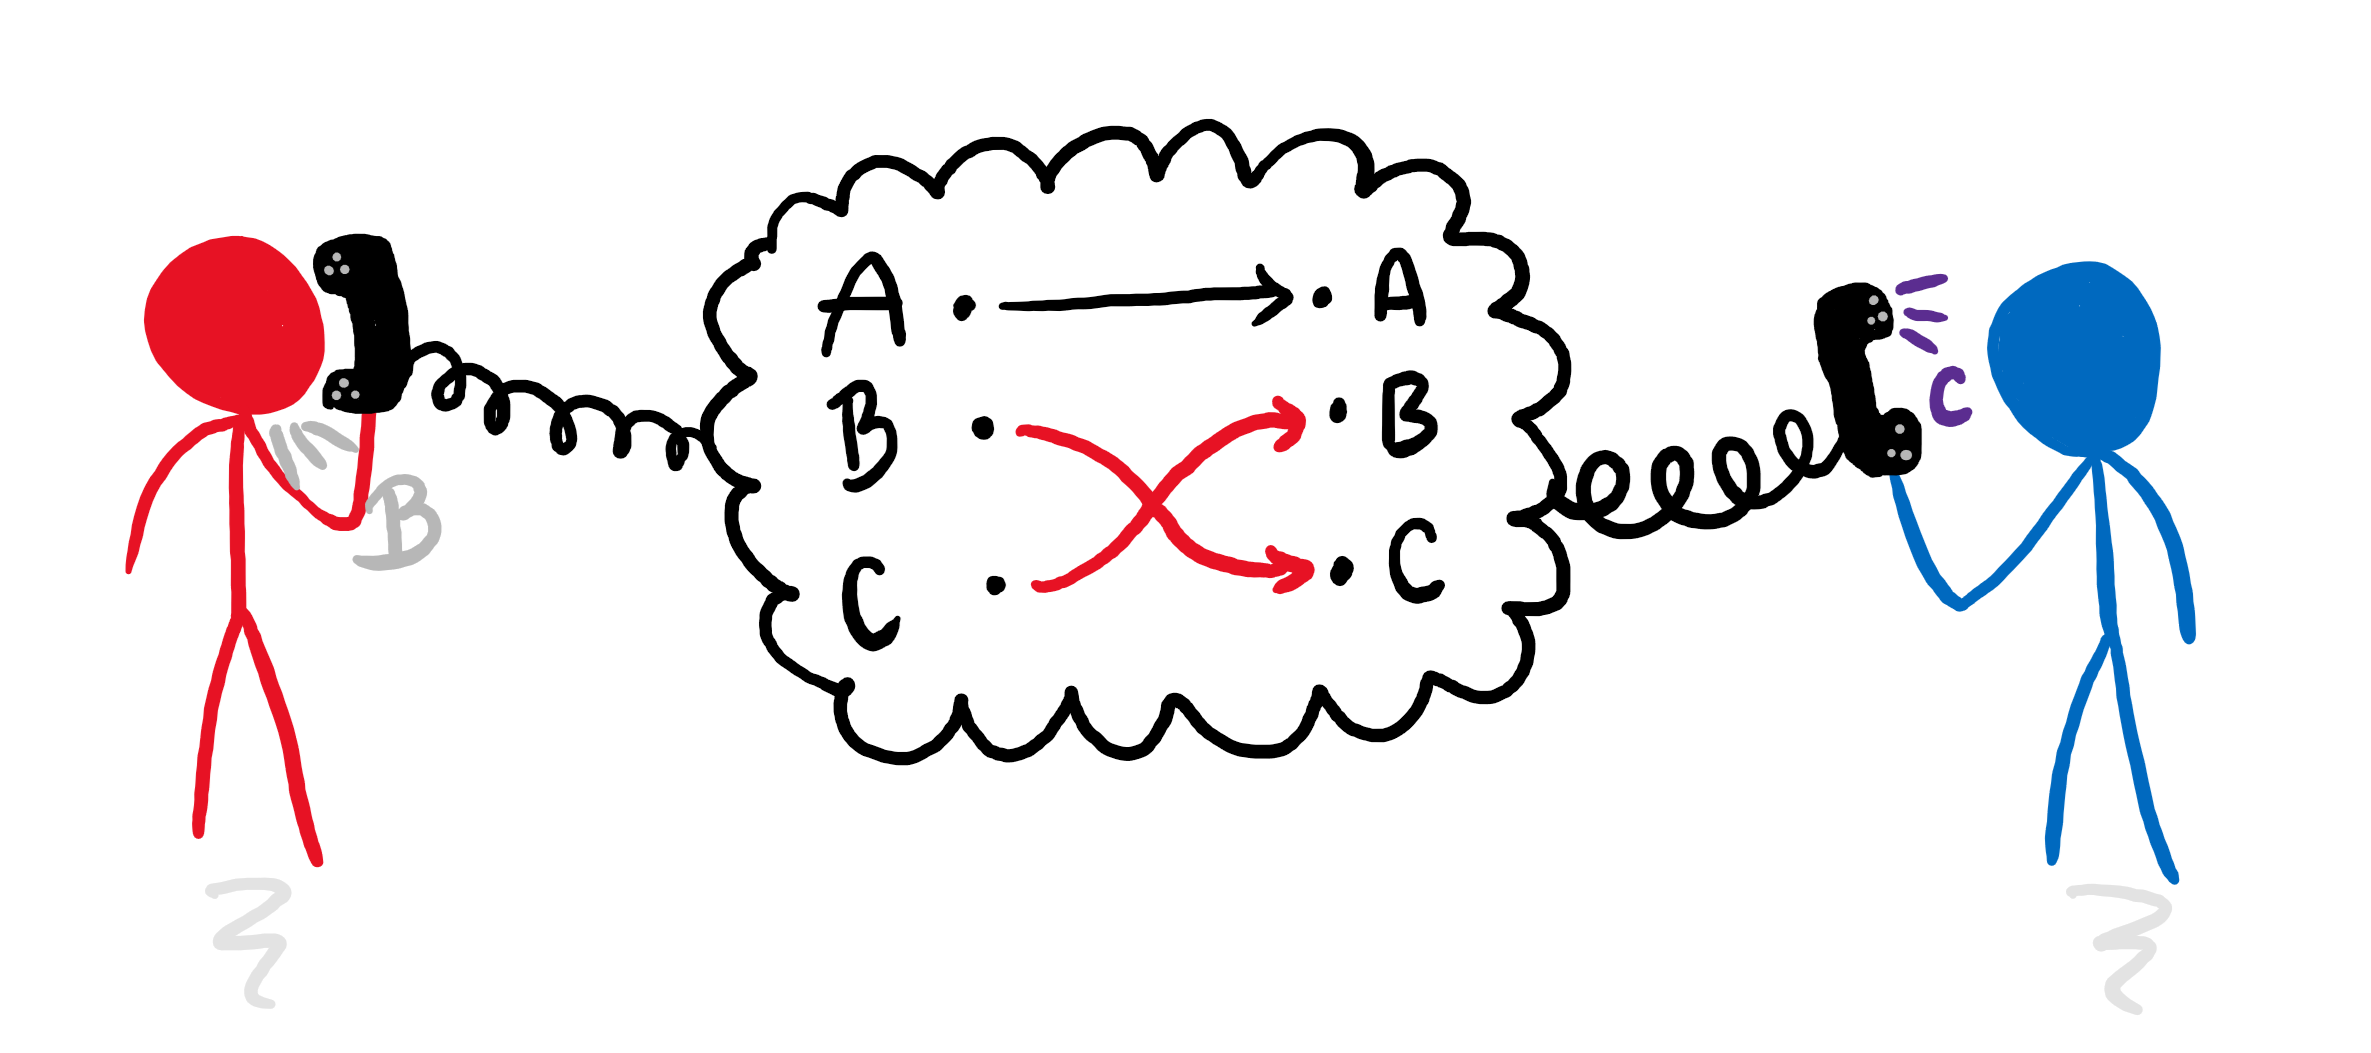
\includegraphics[width=0.8\linewidth]{figures/chan_perm_cartoon.png}
    \end{center}

\end{frame}

\begin{frame}{Channel Permutation}
    
    \begin{figure}
        \centering
        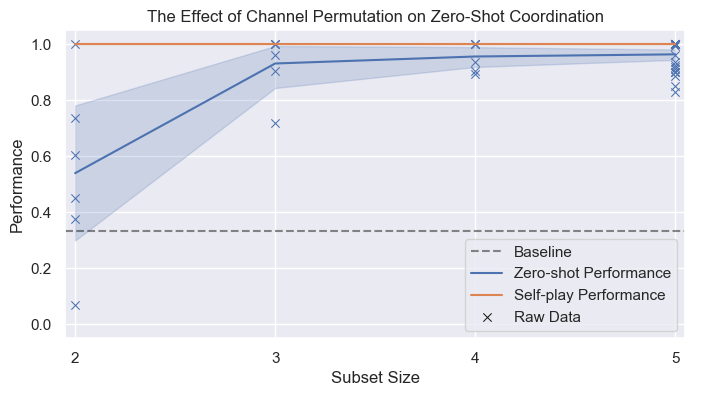
\includegraphics[width=1\linewidth]{figures/permutation_subset_and_zs_coordination.png}
        \caption{Results with varying permutation subset size}
        \label{fig:arch_diagram}
    \end{figure}
    
\end{frame}

\begin{frame}{Conclusions}
    
    \begin{itemize}
        \item Both proposals dramatically improve ZSC
        \item Message mutation assumes a certain set of training signals, and is more sensitive to calibration of $p_m$.
        \item Channel permutation requires fewer assumptions, but is harder to train.
        \item In order to assess the scalability of our proposals, they should be transported to more complex domains. % For channel permutation, this should be a relatively straight-forward implementation. However, for message mutation it is necessary that we can identify where in the episode the protocol ought to be established, i.e.the protocol establishment phase.
    \end{itemize}
\end{frame}